\documentclass[12pt,letterpaper,fleqn]{article}

%       amslatex provides nice math extensions for typesetting mathematics
\usepackage{amsmath}
\usepackage{amsfonts}
\usepackage{tmmaths}
\usepackage{sympytex}

%       pstricks provides powerful environments for incorporating postscript into a
%       TeX/LaTeX document. You must have a postscript printer and a package like
%       dvips to convert the DVI file to a PS file.
%\usepackage{pst-all}
%\usepackage{pstricks,pst-plot}
%\usepackage{pst-coil,pst-node}

%  This package provides native tex support for numbered grids. The syntax is:
%  \graphpaper[spc](x_lowleft,y_lowleft)(x_upperright,y_upperright)

%\usepackage{graphpap}
%\usepackage{float}

%  The package below must be initialized with "\initfloatingfigs" immediately after the
%  "\begin{document} command.
%\usepackage{floatfig}

\usepackage{graphicx}
\graphicspath{{i:/mytex/graphics}}
\DeclareGraphicsExtensions{.ps,.eps}

%       tst is a package for the creation of exams, quizzes and tests. the include
%       file mathstuf (see below) provides many abbreviations for these environments.
%\usepackage{tst}

%       epsfig is a package which provides for the inclusion of Encapsulated PostScript
%       files in a document.
%\usepackage{epsfig}
%\usepackage{epic,eepic}
\include{mathstuf}
\usepackage[total={7.25in,10in},top=0.25in,left=0.75in,includehead]{geometry}
\usepackage{fancyhdr}
\pagestyle{fancy}
\lhead{Math 252}
\rhead{\large Name\makebox[2in]{\hrulefill}}
\chead{\LARGE Exploration 9}
%\lfoot{\today}
\cfoot{}
%\rfoot{\thepage}
\renewcommand{\headrulewidth}{0.4pt}
\renewcommand{\footrulewidth}{0.4pt}
\setlength{\parindent}{0pt}
\setlength{\parskip}{2ex}

\newcounter{tf}[enumi]
\newenvironment{tf}[0]{\begin{list}%
{\alph{tf}. \makebox[5em]{True\hfill False}}%
{\usecounter{tf}\setlength{\labelwidth}{7em}%
\setlength{\leftmargin}{3.5cm}%
\setlength{\labelsep}{1cm}}}%
{\end{list}}

%\usepackage{epic,eepic}
\newcommand{\numline}{%
%\newcounter{mark}%
%\setcounter{mark}{-1}%
\setlength{\unitlength}{0.1in}%
\begin{picture}(0,0)%
\thicklines%
\put(0,0){\line(1,0){60}}%
\multiput(0,0)(10,0){7}{\line(0,-1){1}%
\makebox(0,-1.5)[t]{\arabic{mark}}\stepcounter{mark}}%
%
\thinlines%
\multiput(0,0)(5,0){12}{\line(0,-1){0.5}}%
\multiput(0,0)(1,0){60}{\line(0,-1){0.3}}%
%\put(-5,265){\makebox(0,0)[l]{{\bf cm}}}%
\end{picture}}%

\newcommand{\ds}{\displaystyle}
\usepackage{amsfonts}


\let\oldhat\hat
\renewcommand{\hat}[1]{\oldhat{\boldsymbol{\mathbf{#1}}}}
\newcommand{\lv}[1]{\ensuremath{\langle #1 \rangle}}
\renewcommand{\i}{\ensuremath{\hat{\imath}}}
\renewcommand{\j}{\ensuremath{\hat{\jmath}}}
\renewcommand{\k}{\ensuremath{\mathbf{\oldhat{k}}}}
\newcommand{\ora}[1]{\ensuremath{\overrightarrow{#1}}}
\renewcommand{\vec}[1]{\ensuremath{\mathbf{#1}}}
\renewcommand{\v}[1]{\ensuremath{\vec{#1}}}
\newcommand{\abs}[1]{\ensuremath{\lvert #1 \rvert}}

\usepackage{tabularx}
\usepackage{paralist}
\newcommand{\red}[1]{\textcolor{red}{#1}}
\newcommand{\blue}[1]{\textcolor{blue}{#1}}
% \newcommand{\ans}[1]{\quad\fbox{answer: \red{#1}}}
\newcommand{\ans}[1]{\mbox{{\bf Ans:} \blue{#1}}}
\newcommand{\dd}[2][]{\ensuremath{\frac{\text{d}#1}{\text{d}#2}}}
\newcommand{\eval}[2]{\ensuremath{\left.#1\right|_{#2}}}

\usepackage{amsthm}

\theoremstyle{definition}
\newtheorem*{definition}{Definition}


\begin{document}
\section*{Work in Physics}
In this exploration we consider the concept of ``work'' as understood in Physics. The science of Physics seeks to understand nature through the action of forces (pushes and pulls) on objects. Work has to do with how forces act on objects so as to move them through some distance.

\begin{definition}
 The work $W$ done done by a constant force $F$ on an object in moving it a distance $d$ in the direction of the force is defined as $W = Fd$.
\end{definition}

Forces and distances are typically measured in either metric units or imperial units. In metric units forces are measured in Newtons (N) and distances in meters (m). In imperial units forces are measured in pounds (lbs) and distances in feet (ft). One Newton is the amount of force required to accellerate a 1 kilogram mass at a rate of 1 $\text{m/s}^2$ (its velocity increases by 1 meter per second each second). Therefore, the units of force in imperial units are ``foot pounds'' (ft-lbs) and the units of force in metric units are ``Newton meters'' (N-m) also called ``Joules'' (J).

For example, if a constant force of 5 pounds acts horizontally on a book resting on a table so as to move it a distance of 3 feet, then the work done by the force on the book is $W = 5\text{ pounds} \cdot 3\text{ feet} = 15 \text{ ft-lbs}$.

\begin{enumerate}
  \item Consider the variable force depicted in the graph below. Find:
  \begin{enumerate}
    \item The work done in moving an object from $x=0$ to $x=5$. Include correct units.
    \item The work done in moving the object from $x=4$ to $x=9$. Include correct units.
    \item The work done in moving the object from $x=0$ to $x=10$. Include correct units.
  \end{enumerate}
  \begin{figure}[!htb]
	\centering
	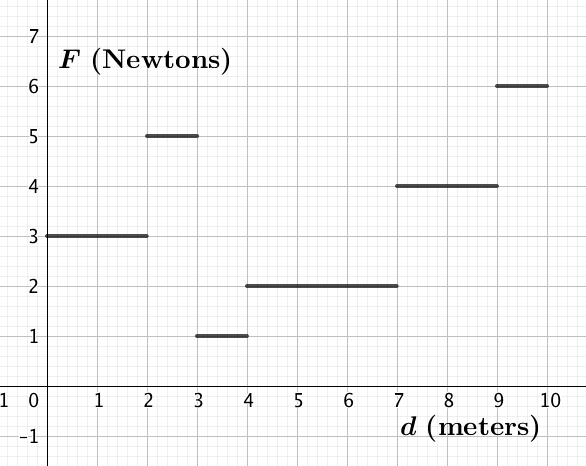
\includegraphics[width=0.5\textwidth]{img/variable_force.png}
	% \caption{}
	% \label{}
\end{figure}
\newpage
\item Consider the continuously varying force depicted in the graph below. Imagine partitioning the interval $[0,5]$ into a very large number of subintervals of width $dx$ and approximating the varying force over each subinterval with a constant force $F(x)$, where $x$ is in that subinterval.
\begin{enumerate}
  \item What expression represents the work done by the force on an object in moving the object over such a subinterval?
  \item Write an integral representing the total work done by the force $F(x)$ on an object in moving that object over the whole interval $[0,5]$
  \item Suppose the force is given by $F(x) = \dfrac{6}{x+1}$, for $0\leq x\leq 5$, where $F$ is measured in pounds and $x$ is measured in feet. Set up and evaluate a definite integral representing the work done by this force $F$ in moving an object from $x=0$ to $x=5$.
\end{enumerate}
\begin{figure}[!htb]
	\centering
	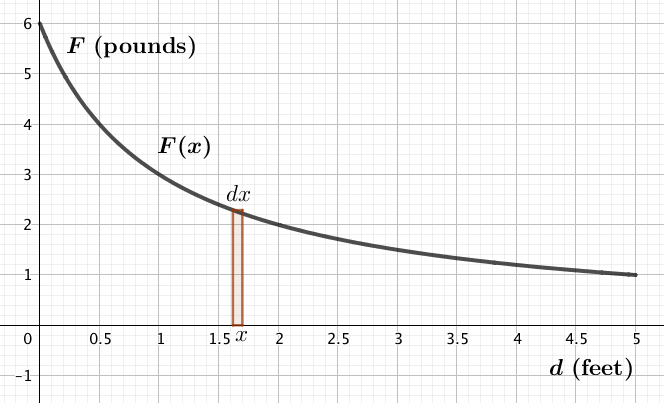
\includegraphics[width=0.5\textwidth]{img/continuous_force.png}
	% \caption{}
	% \label{}
\end{figure}
\end{enumerate}
\end{document}
